\documentclass[tikz,border=5pt]{standalone}
\usepackage{amsmath,amssymb}
\usetikzlibrary{shapes.geometric, arrows.meta, positioning, calc}

\begin{document}
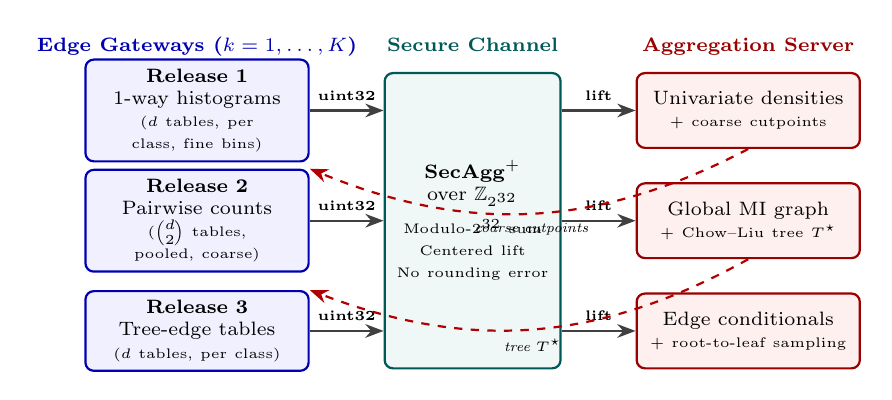
\begin{tikzpicture}[
    font=\scriptsize, >=Stealth,
    cbox/.style={rectangle, draw=blue!70!black, fill=blue!6, rounded corners=3pt, thick, text width=2.6cm, minimum height=0.95cm, align=center},
    sbox/.style={rectangle, draw=red!60!black, fill=red!6, rounded corners=3pt, thick, text width=2.6cm, minimum height=0.95cm, align=center},
    arr/.style={->, thick, draw=black!75},
    lbl/.style={font=\tiny\bfseries, above}
]
\node[cbox] (c1) at (0, 0)    {\textbf{Release 1}\\1-way histograms\\{\tiny ($d$ tables, per class, fine bins)}};
\node[cbox] (c2) at (0, -1.4) {\textbf{Release 2}\\Pairwise counts\\{\tiny ($\binom{d}{2}$ tables, pooled, coarse)}};
\node[cbox] (c3) at (0, -2.8) {\textbf{Release 3}\\Tree-edge tables\\{\tiny ($d$ tables, per class)}};

\node[rectangle, draw=teal!70!black, fill=teal!6, rounded corners=3pt, thick, text width=2.0cm, minimum height=3.75cm, align=center] (sa) at (3.5, -1.4) {\textbf{SecAgg}$^+$\\over $\mathbb{Z}_{2^{32}}$\\[4pt]{\tiny Modulo-$2^{32}$ sum}\\{\tiny Centered lift}\\{\tiny No rounding error}};

\node[sbox] (s1) at (7.0, 0)    {Univariate densities\\{\tiny + coarse cutpoints}};
\node[sbox] (s2) at (7.0, -1.4) {Global MI graph\\{\tiny + Chow--Liu tree $T^\star$}};
\node[sbox] (s3) at (7.0, -2.8) {Edge conditionals\\{\tiny + root-to-leaf sampling}};

\node[font=\scriptsize\bfseries, text=blue!70!black, anchor=base] at (c1 |- 0, 0.75) {Edge Gateways ($k = 1, \dots, K$)};
\node[font=\scriptsize\bfseries, text=teal!70!black, anchor=base] at (sa |- 0, 0.75) {Secure Channel};
\node[font=\scriptsize\bfseries, text=red!60!black, anchor=base] at (s1 |- 0, 0.75) {Aggregation Server};

\foreach \i in {1,2,3} {
    \draw[arr] (c\i.east) -- node[lbl] {uint32} (sa.west |- c\i.east);
    \draw[arr] (sa.east |- s\i.west) -- node[lbl] {lift} (s\i.west);
}

% Dotted arrows from server back to gateways
\draw[->, thick, dashed, draw=red!70!black] (s1.south) to[bend left=25] node[below, font=\tiny\itshape] {coarse cutpoints} (c2.north east);
\draw[->, thick, dashed, draw=red!70!black] (s2.south) to[bend left=25] node[below, font=\tiny\itshape] {tree $T^\star$} (c3.north east);

\end{tikzpicture}
\end{document}
